\section{Internal Pages}
In this section we are analizing a macro category (the same works for subcategories)

\subsection{Informative axes}
The informative axes' observations are similar to what is written in section \ref{6w},
but the page has changed a little bit. In fact there are no element for asnwering to
"\textit{when}" or "\textit{why}" questions. Still these informations can be omitted
because they are not as important as the other ones.

\subsection{Advanced Search}
The website make available some advanced features for searrching in a more accurate way.\\
There are different types of parameters and the filter action is dynamic, so every chosen
constraint triggers an new search update. Actually this method can be useful for incremental searches,
but not for focused ones.\\
One bad aspect is that the filtering buttons are displayed vertically and not horizontally.
This implies to steal some horizontal space that could be used  to better organize products disposition.
Moreover filter's buttons are more visible for the F-shape map and that is not the goal. In fact the focus of the user should be more
about products than filter's buttons (figure \ref{internal-adv-search}).

\begin{figure}[!h] 
    \centering 
    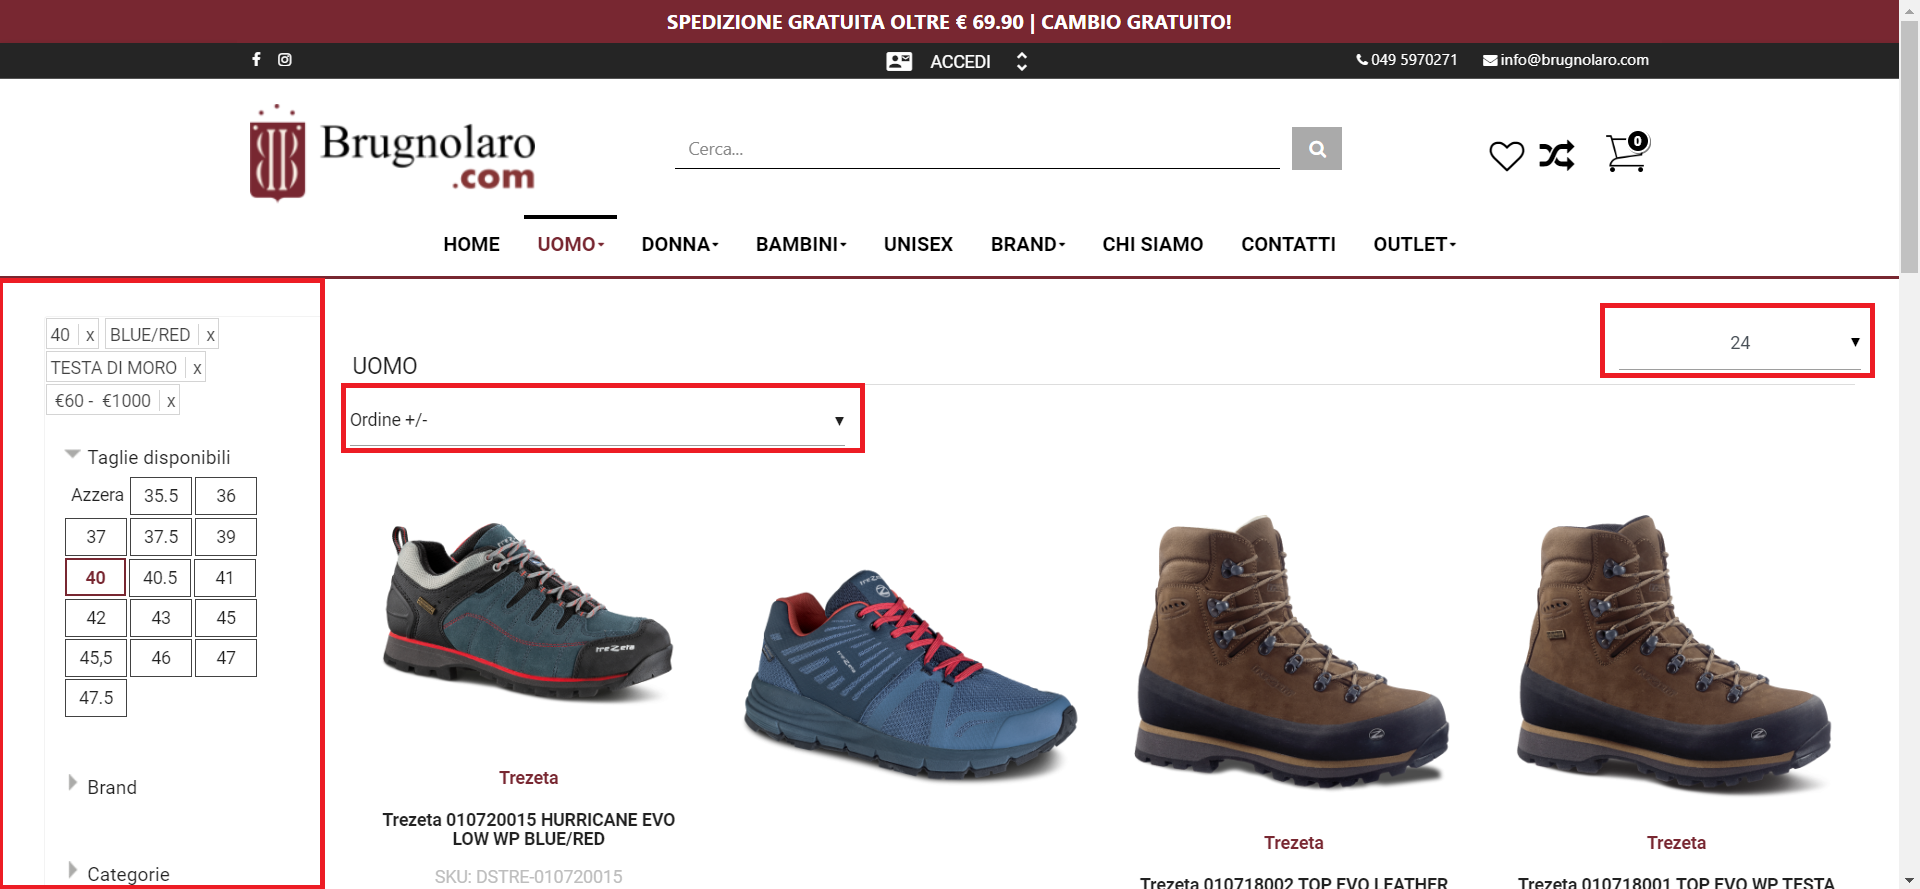
\includegraphics[scale = 0.29]{images/adv_search.png} 
    \caption{Internal page (advanced search)}
    \label{internal-adv-search}
\end{figure}
\newpage
\subsection{Search Results}
Results is actually the output which is displayed to the user satisfying his preferences.

So the presentation is a grid and each line contains 4 products. This disposition is working
on 2 dimensions and so implies more computational effort.

It is not clear why there is no title about product's number filter
(how do you know that? Gambling click). This may lead some confusion to the user.

Then the ordering results functionality is not done in a good way. In fact it is
very difficult to understand how to go from ascendent to descendent ordering.
Clicking on the select box for changing the ordering in the opposite way is not
the easiest and intuitive way for the user.

About the items in the grid presentation, they are very good. Infact there is a 2D image with near its name, its price
and also its available sizes. In particular the last information can be very useful in order to navigate without
using size filter which could be annoying because of dynamic search.

If there are no results during the searching, "No results" string will be displayed which is fine
(figure \ref{internal-no-results}).
\vspace*{\fill}
\begin{figure}[!h] 
    \centering 
    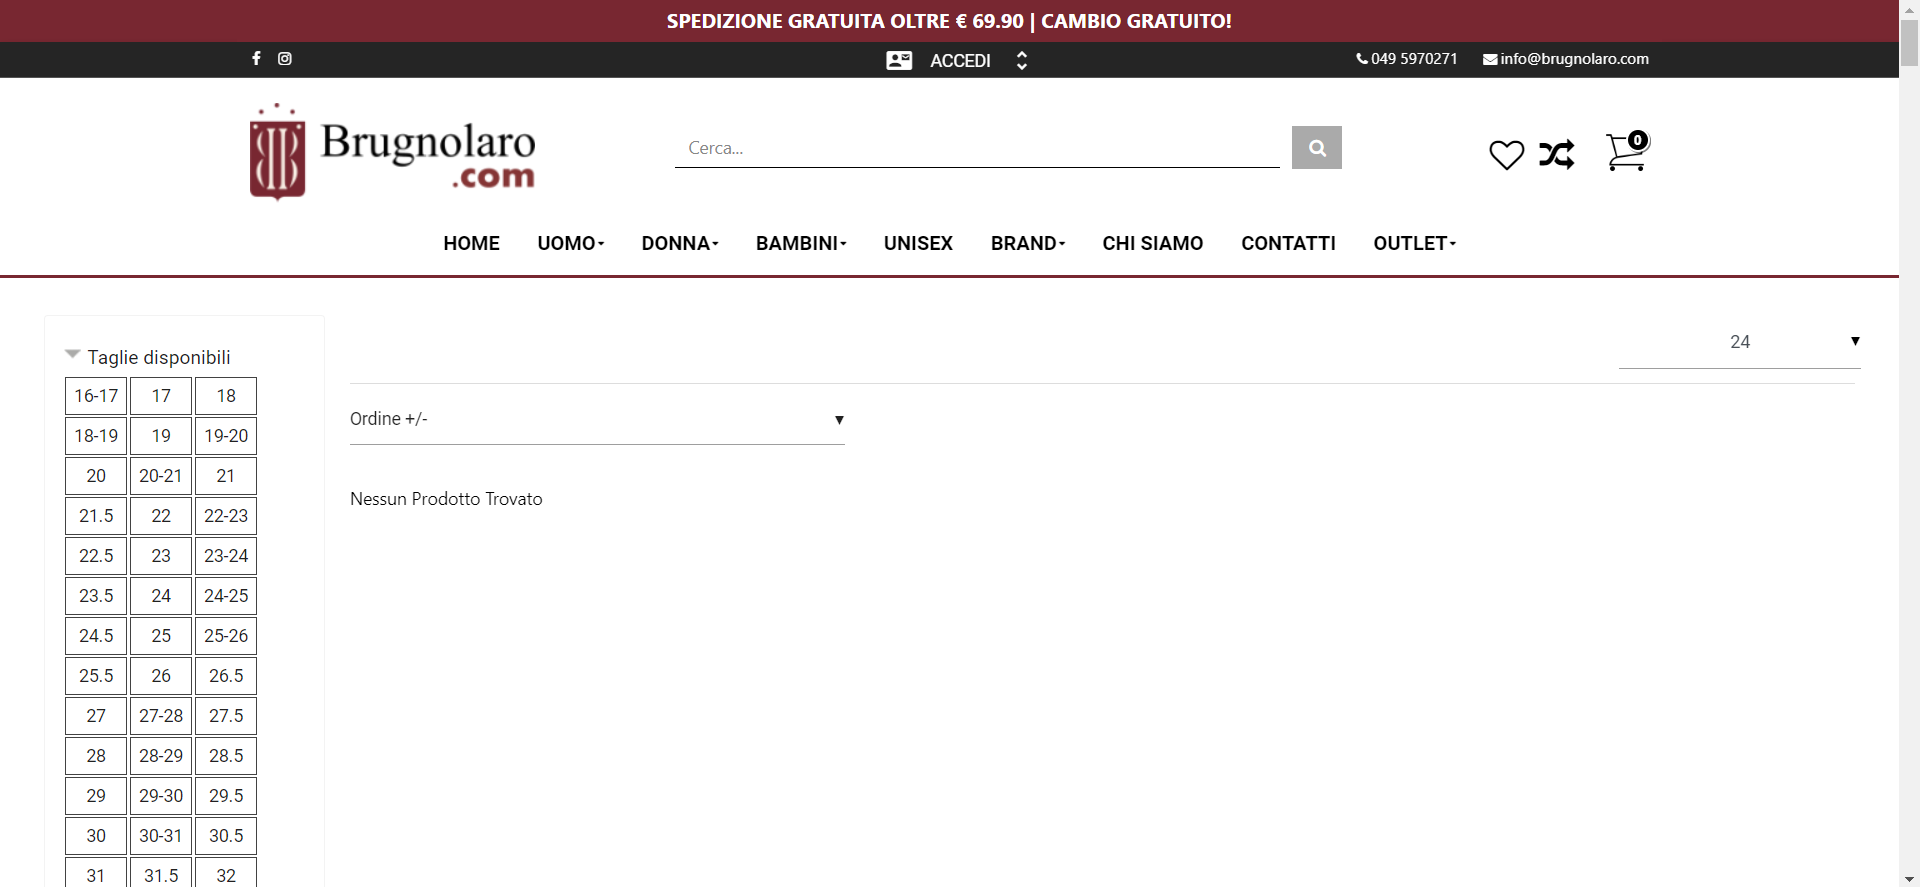
\includegraphics[scale = 0.29]{images/no_results.png} 
    \caption{Internal page (no results)}
    \label{internal-no-results}
\end{figure}
\vspace*{\fill}
\newpage
\subsection{Product}
This subsection aims to analyze the way in which the product is presented.
The best layout of a product webpage of an e-commerce should contain the following components:
\begin{itemize}
    \item Product's visual description (images, videos): allows user to see the product;
    \item Product's textual description: provides description of the product's features;
    \item Price: useful for making product-price association;
    \item Cart: presence of the ”Add to cart” button.
\end{itemize}

\subsubsection{Visual Description}
The images are in 2 dimension, which is really good. In fact this allows the users not
to interact with a 3 dimensional object which leads to more computation effort.

The user can also interact with the image and this
is a good design choice.
There is the zoom functionality which allows the user to better observe the
product's details (figure \ref{internal-zoom}).
\begin{figure}[!h] 
    \centering 
    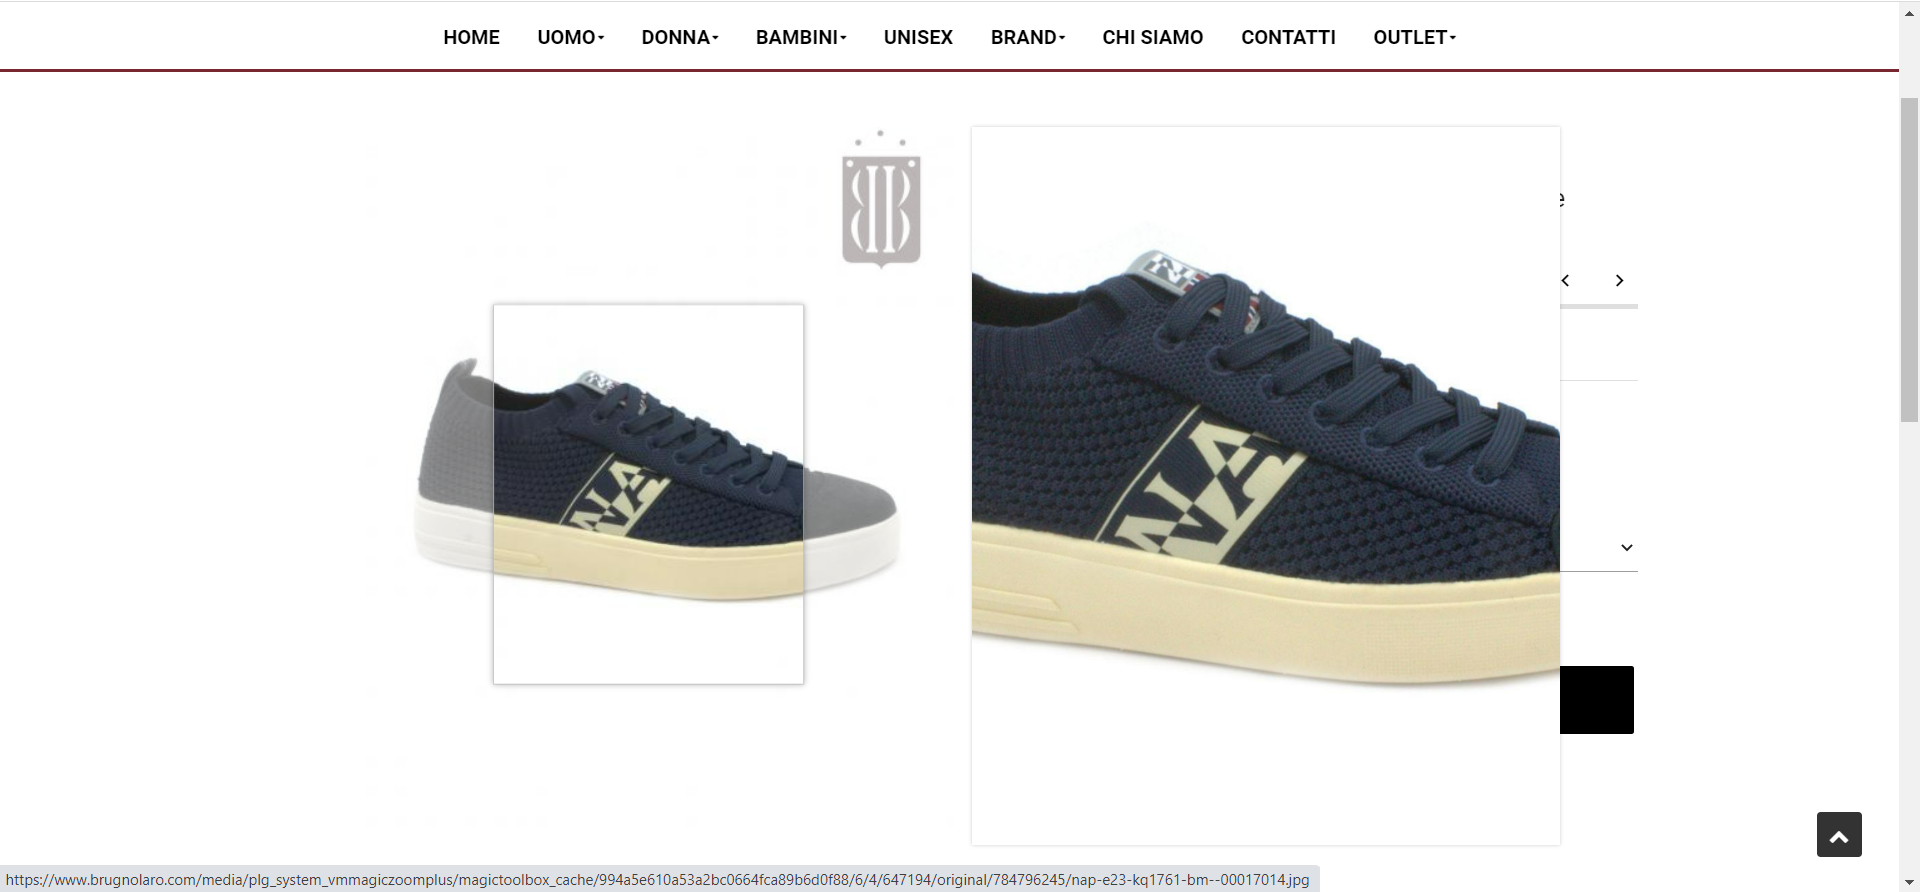
\includegraphics[scale = 0.29]{images/zoom_product.png} 
    \caption{Internal page (zoom functionality)}
    \label{internal-zoom}
\end{figure}
\newline
A bad choice is writing how to zoom.
In particular, saying "\textit{use scroll in order to increase/decrease zoom}" is wrong because
many users could not use a mouse but the laptop's trackpad (figure \ref{internal-product}).
\begin{figure}[!h] 
    \centering 
    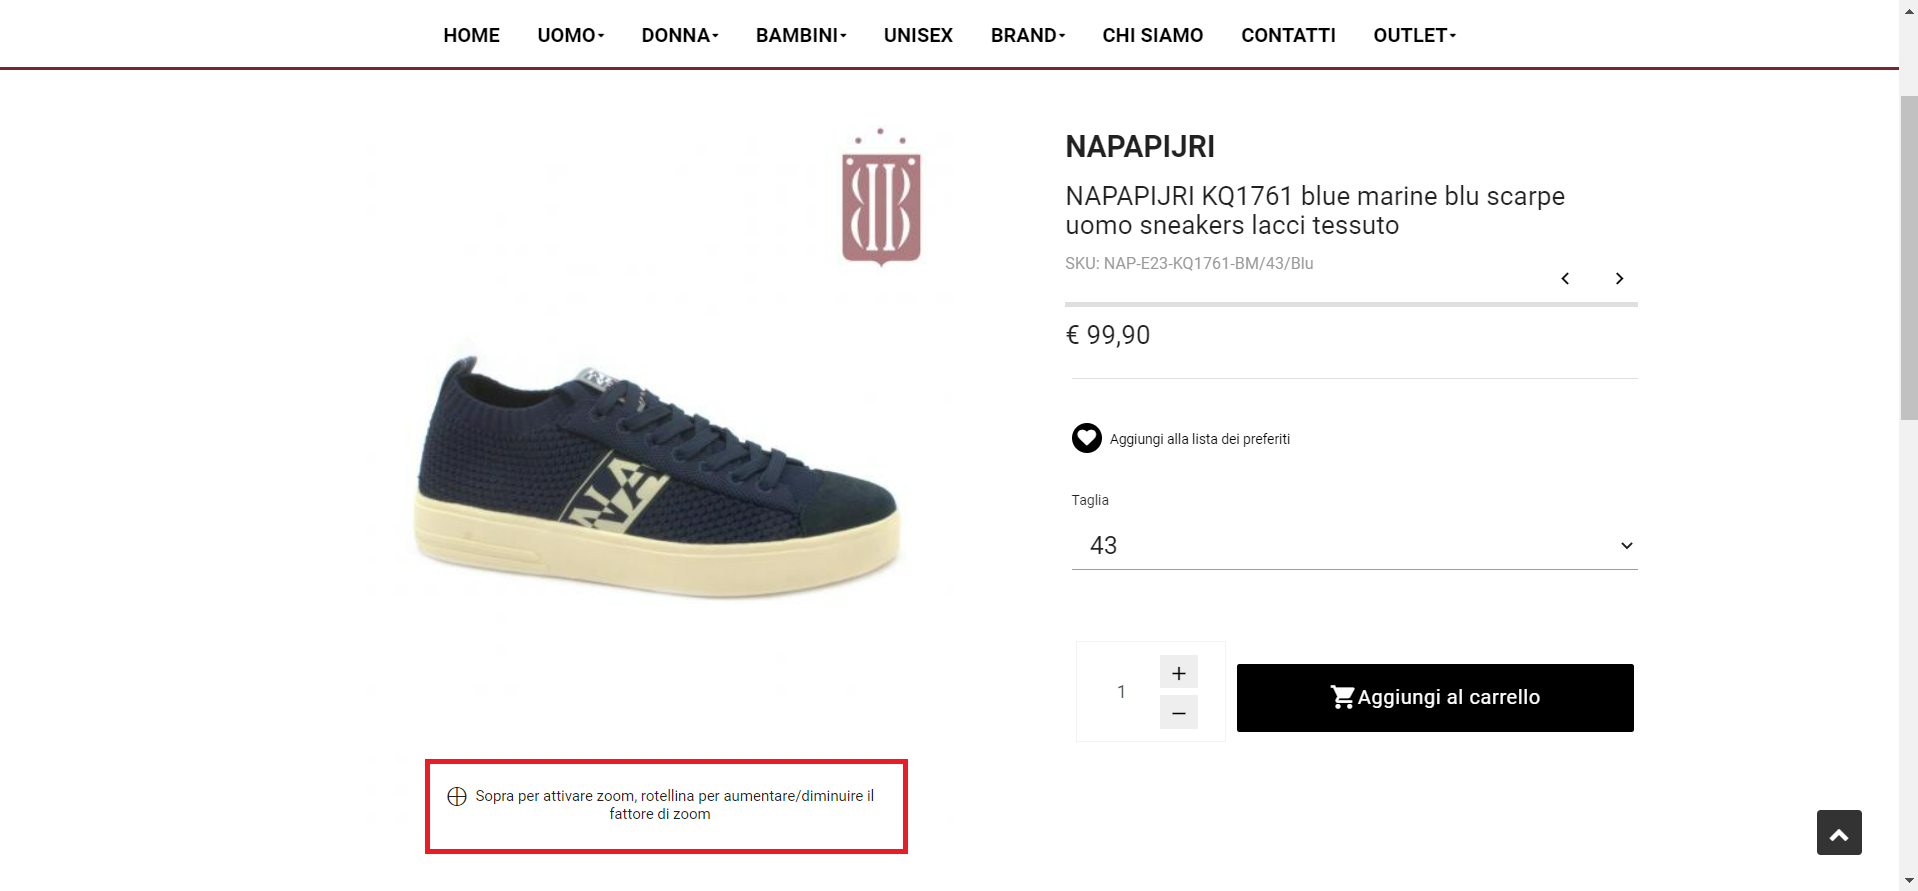
\includegraphics[scale = 0.29]{images/product_price.png} 
    \caption{Internal page (product)}
    \label{internal-product}
\end{figure}
\newpage
It is also good the possibility for the user to open the image in fullscreen page in order to better
see it (figure \ref{internal-opened-image})
\begin{figure}[!h] 
    \centering 
    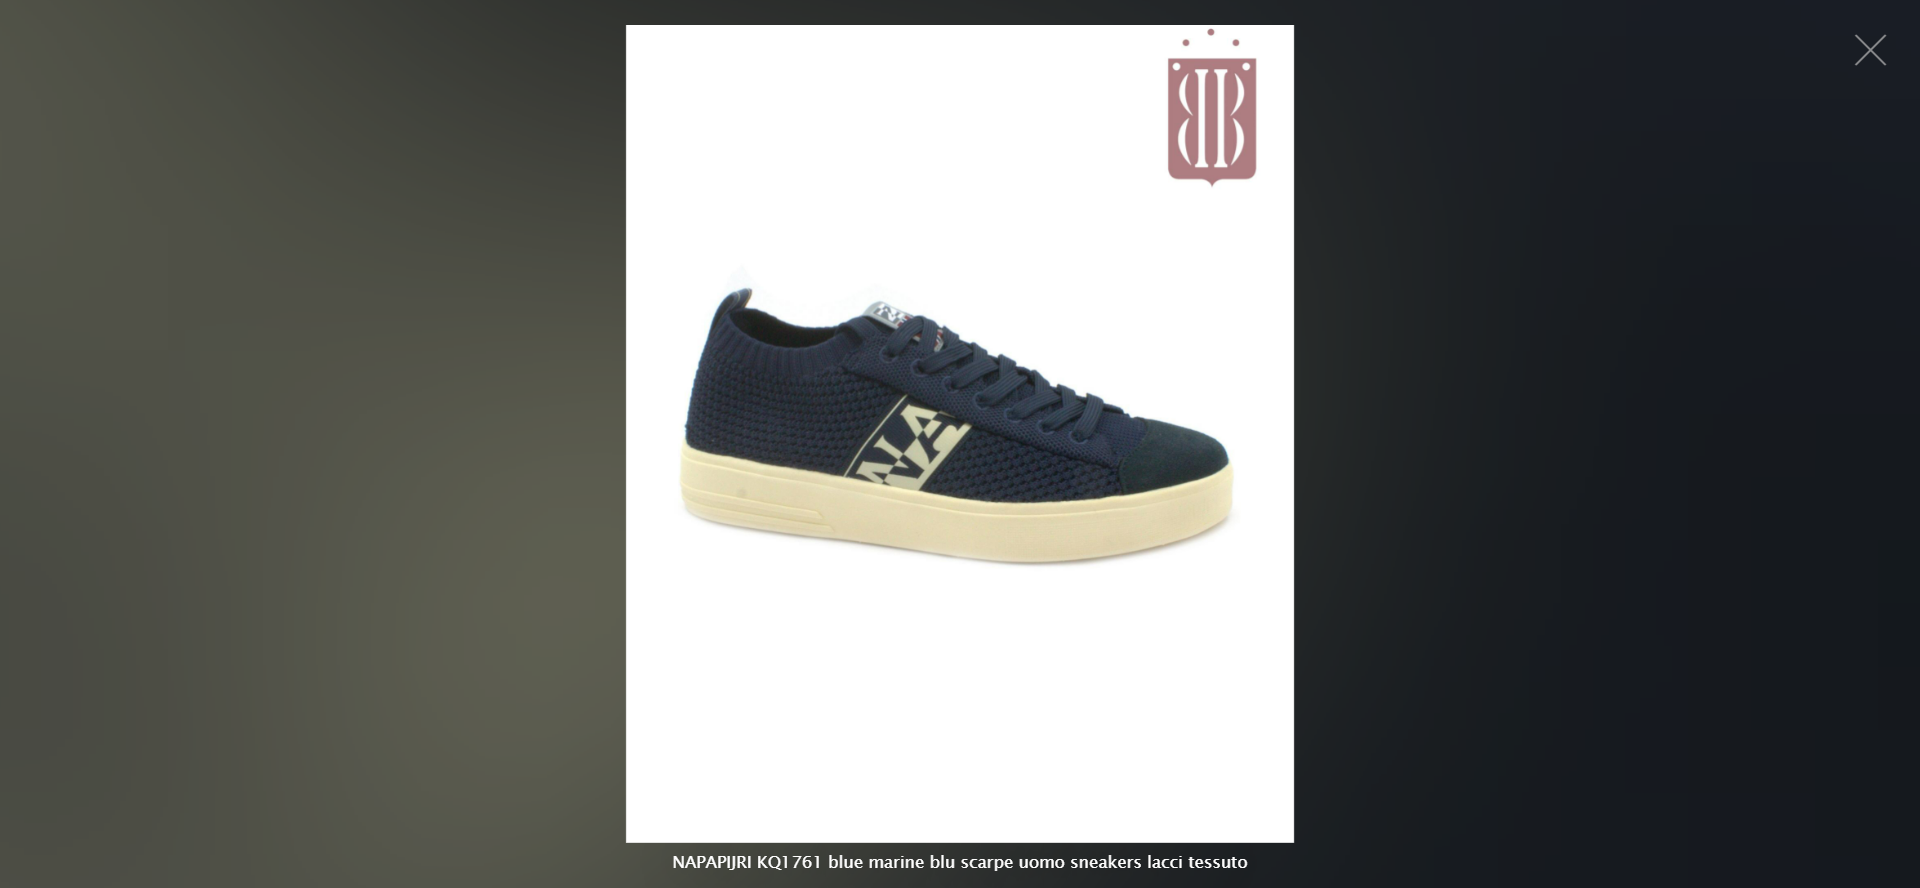
\includegraphics[scale = 0.29]{images/open_image_product.png} 
    \caption{Internal page (opened image)}
    \label{internal-opened-image}
\end{figure}
\newline
So finally images are designed in a good way but there is the need to solve that \mbox{problem} about the zoom
functionality.

\newpage
\subsubsection{Textual Description}
The textual description is very important because the user has to know about specific
characterisitics about the product. It is suggested to put it before the "\textit{Add to cart}" button.
This because most of hte people think that after that button there is nothing important.
If there is no description the user classify your shop like if you want to hide something
which is bad about the product.
In this case the position of the textual description is wrong because is under the button
(figure\ref{internal-specifics})
\begin{figure}[!h] 
    \centering 
    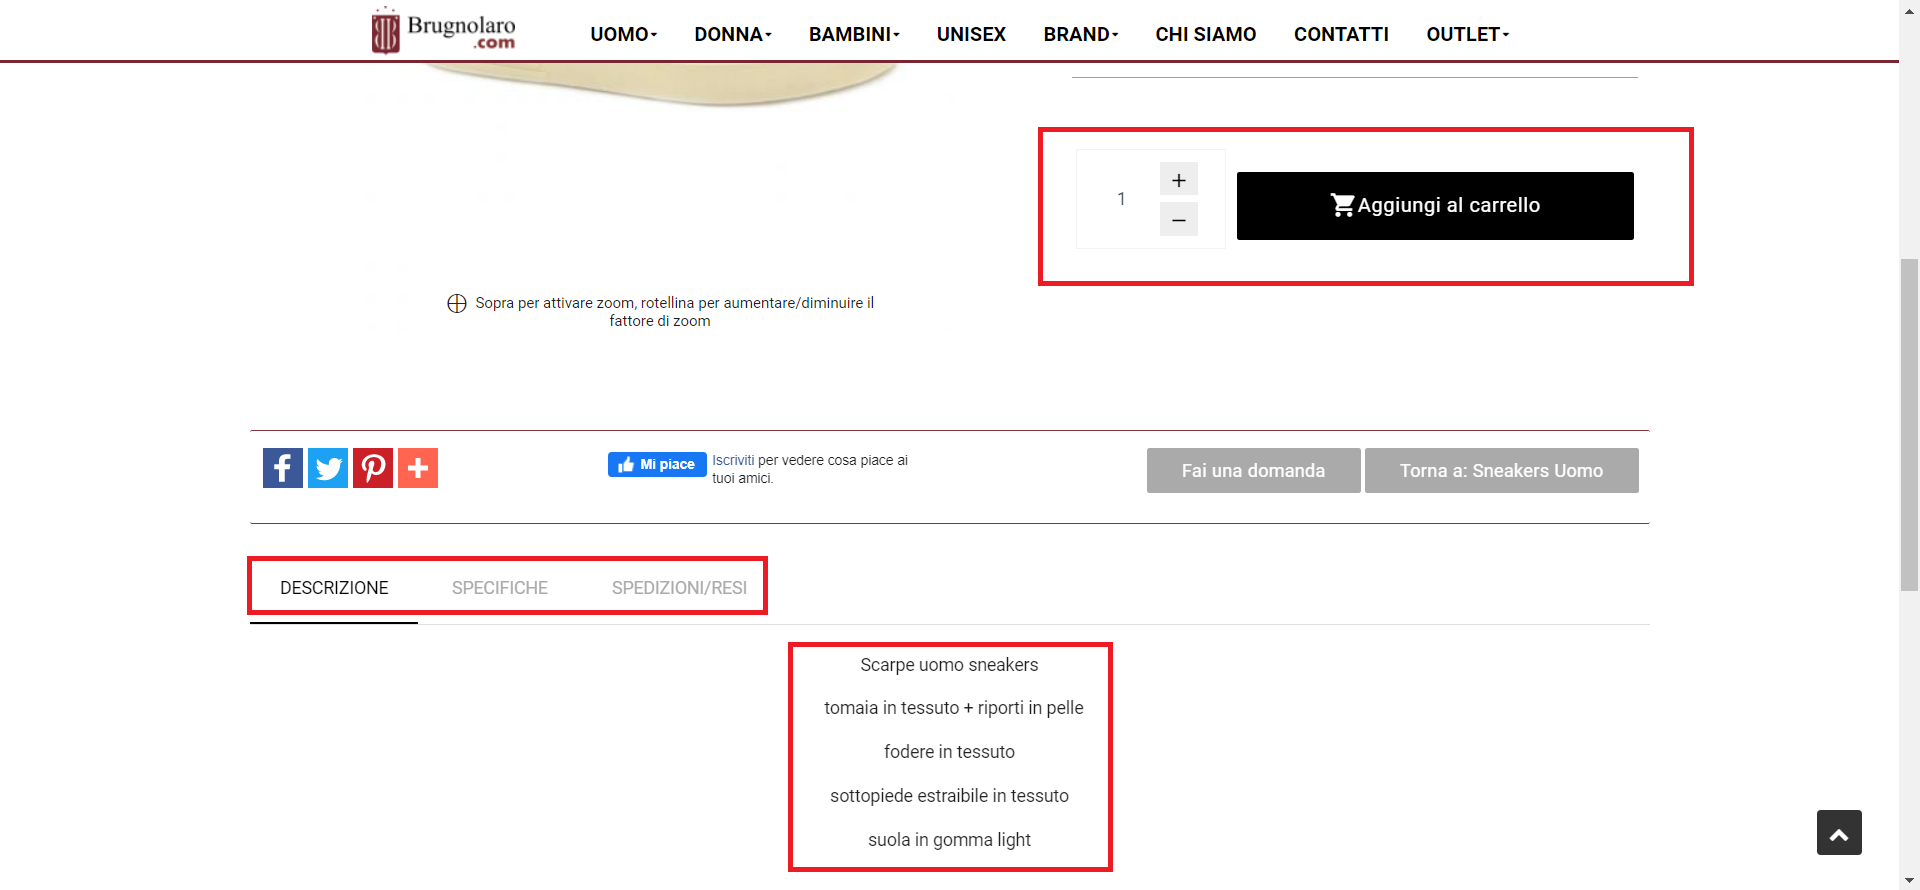
\includegraphics[scale = 0.29]{images/product_specifics.png} 
    \caption{Internal page (product's specifics)}
    \label{internal-specifics}
\end{figure}

\subsubsection{Price}
The price is always visible and it is positioned under the name of it. This is a good design choice because
users are used to associate the position of the price near the name of the product (figure \ref{internal-product}).
\newpage
\subsection{Checkout}
In the checkout page there is each product which is associated with its price. That is
really good and clever, because users are not required to remember prices and this can decrease the computational
effort done by the user.
A bad choice is that an account registration is required while performing the checkout.
In section §\ref{ask-personal-data} there is no evidence of requests of personal data
for visiting the website. However in this section of the website the condition
of giving data is very bad and the user could lose the trust on the website (figure \ref{internal-checkout}).

\begin{figure}[!h] 
    \centering 
    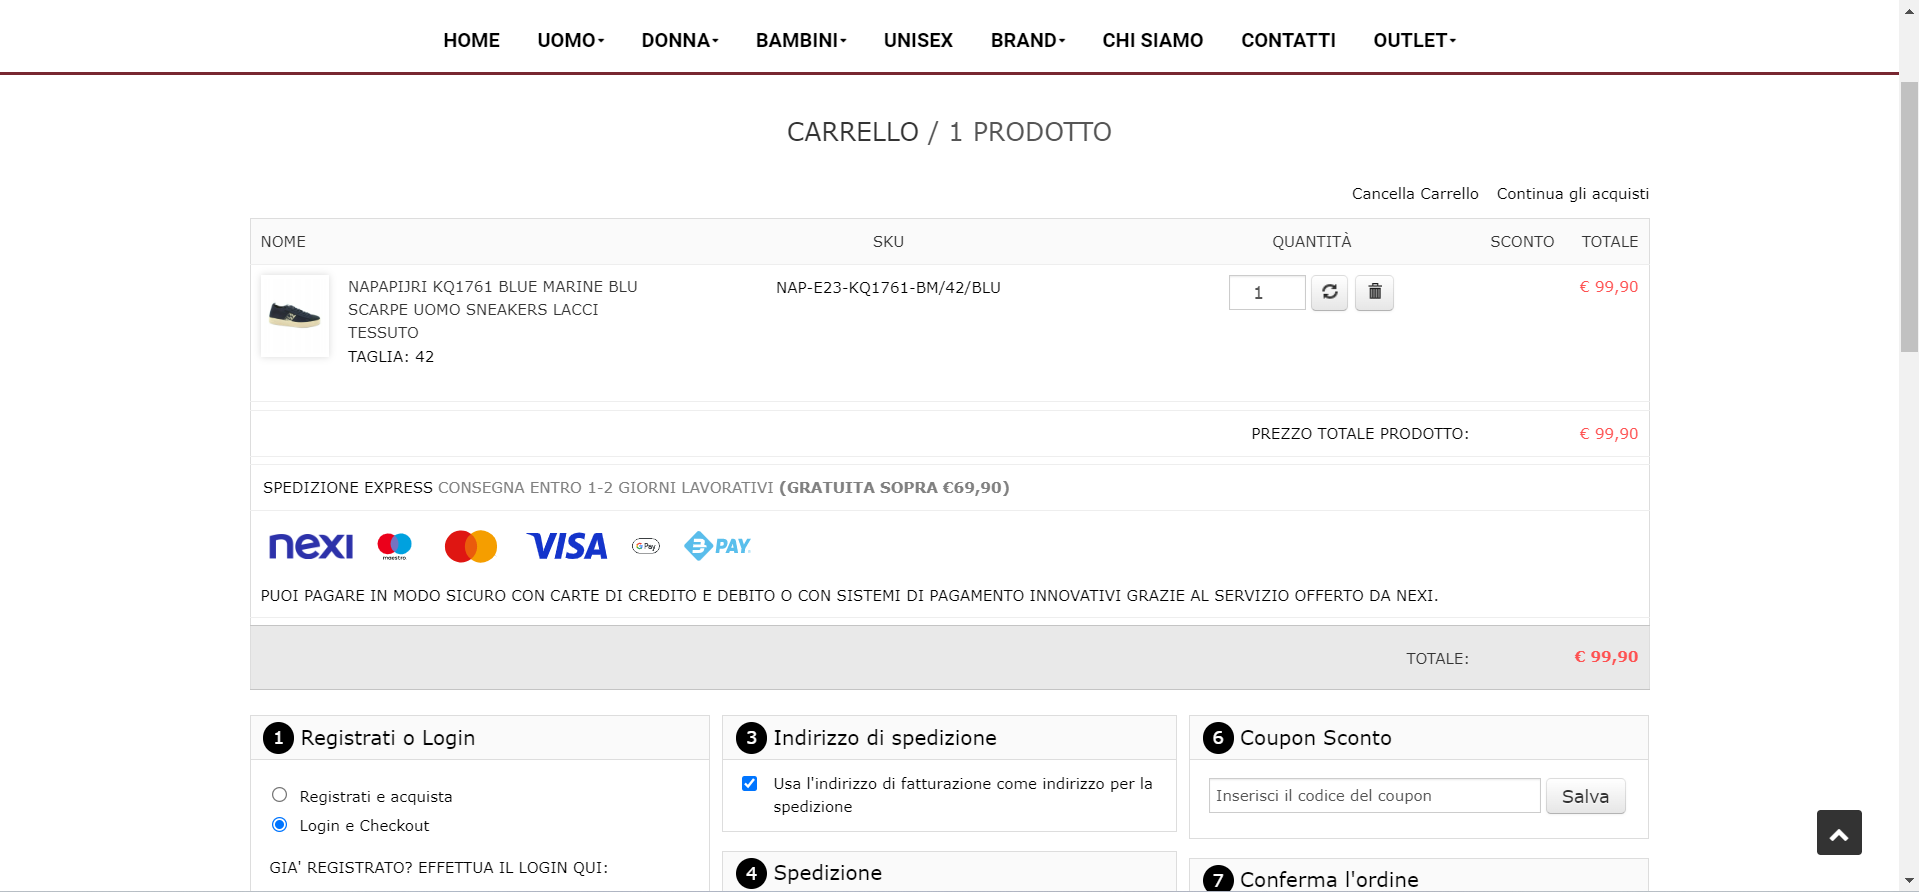
\includegraphics[scale = 0.29]{images/checkout.png} 
    \caption{Internal page (checkout)}
    \label{internal-checkout}
\end{figure}

